\section{A very simple example - polynomial curve fitting}\label{sec:simple}
\subsection{The first program in C++}
{\em Example file polyfit0.cpp in the directory doc/tutorial/code/polyfit.}\\
Let us start with the very simple inverse problem of fitting a polynomial curve of degree $P$
\[ f(x) = p_0 +p_1 x + \ldots + p_P x^P= \sum\limits_{i=0}^{P} p_i x^i \]
to some existing data $y$. The unknown model is the coefficient vector $\m=[p_0,\ldots,p_P]$.
The vectorized function for a vector $\bf x=[x_1,\ldots,x_N]^T$ can be written as matrix-vector product
\begin{equation}\label{eq:yAx}
  \f(\x) = \A \x \quad\mbox{with}\quad \A=\left[ \begin{array}{cccc}
  1 & x_1 & \ldots & x_1^P \\ \vdots & \vdots & \ddots & \vdots \\ 1 & x_N & \ldots & x_N^P
  \end{array} \right] = [ {\bf 1}\quad \x \quad \x^2 \ldots \x^P ] \quad.
\end{equation}

We set up the modelling operator, i.e. to return $\f(\x)$ for given $p_i$, as a class derived from the modelling base class. The latter holds the main mimic of generating jacobian, gradients by brute force. The only function to overwrite is \cw{response()}.

\begin{lstlisting}[language=C++,morekeywords={RVector,ModellingBase}]
class FunctionModelling : public ModellingBase {
public:
    /*! constructor, nc: number of coefficients, xvec: abscissae */
    FunctionModelling( int nc, const RVector & xvec, bool verbose=false )
        : ModellingBase( verbose ), x_( xvec ), nc_( nc ){
        regionManager_->setParameterCount( nc ); //! instead of a mesh
    }
    /*! the main thing - the forward operator: returns f(x) */
    RVector response( const RVector & par ){
        RVector y( x_.size(), par[ 0 ] );   //!constant vector of p0
        for ( size_t i = 1; i < nc_; i ++ ) //! p1 to pP
            y += pow( x_, i ) * par[ i ];   //! add pi*x^i
        return y;                           //! return sum
    }
    /*! define the startmodel */
    RVector startModel( ){ return RVector( nc_, 0.5 ); }
protected:
    RVector x_; //! abscissa vector x
    int nc_; //! number of coefficients
};
\end{lstlisting}

In the constructor the $\bf x$ vector and the number of coefficients are saved as protected variables\footnote{Usually all variables are denoted with an underscore and declared as protected. Instead of accessing the values directly, we use set and get functions that control the validity of the arguments.}.
The function \cw{setParameterCount} setups the parameterisation as a 0d mesh of \cw{nc} unknowns.
The main type used is \cw{RVector}, a vector of real (\cw{double}) values.

We now want to apply the function to the real inversion of data and write a main program.
\begin{lstlisting}[language=C++,morekeywords={RVector,RMatrix,RInversion,EXIT_SUCCESS}]
int main( int argc, char *argv [] ){
    int np = 1; /*! maximum polynomial degree fixed to 1 */
    RMatrix xy; //! two-column matrix from file holding x and y
    loadMatrixCol( xy, "datafile.dat" );
    /*! initialise modelling operator */
    FunctionModelling f( np + 1, xy[ 0 ] ); //! first data column
    /*! initialise inversion with data and forward operator */
    RInversion inv( xy[ 1 ], f );
     /*! the problem is well-posed and does not need regularization */
    inv.setLambda( 0 );
    /*! actual inversion run yielding coefficient model */
    RVector coeff( inv.run() );
    /*! save coefficient vector to file */
    save( coeff, "out.vec" );
    /*! exit programm legally */
    return EXIT_SUCCESS;
}
\end{lstlisting}

The data in the two-column data file is read into a real matrix (\lstinline|RMatrix xy;|) whose columns can be assessed by \lstinline|xy[i]|. We initialise the forward class as defined and the inversion by specifying data and forward operator.
Then any options of the inversion can be set, such as the regularization parameter being zero.

Instead of using a fixed polynomial degree and a pre-defined file name we might specify this by the command line in order to have a user-friendly tool.
For this, an option map is applied reading the last argument and the optionally defined -n switch.
\begin{lstlisting}[language=C++,morekeywords={OptionMap,RMatrix,loadMatrixCol}]
    int np = 1;
    std::string datafile;
    OptionMap oMap;
    oMap.setDescription("Polyfit - fits two-column data with polynomials");
    oMap.addLastArg( datafile, "Datafile" );
    oMap.add( np, "n:", "np", "Number of polynomials" );
    oMap.parse( argc, argv );
    RMatrix xy; 
    loadMatrixCol( xy, datafile );
\end{lstlisting}

The provided datafile \verb|y_2.1x+1.1.dat| holds synthetic noisified data for a linear function.
A call \verb|curvefit -n1 y_2.1x+1.1.dat| yields values close to the synthetic ones.

\subsection{A first Python program}
{\em Example file polyfit.py in the directory doc/tutorial/code/polyfit.}\\
Python is a very flexible language for programming and scripting and has many packages for numerical computing and graphical visualization.
For this reason, we built Python bindings and compiled the library pygimli.
As a main advantage, all classes can be used and derived.
This makes the use of GIMLi very easy for non-programmers.
All existing modelling classes can be used, but it is also easy to create new modelling classes.

We exemplify this by the preceding example.
First, the library must be imported.
To avoid name clashes with other libraries we suggest to import it to an easy name, e.g. by using \lstinline|import pygimli as g|.
As a result, all gimli objects (classes and functions) can be referred to with a preceding \lstinline|g.|, e.g. \lstinline|g.RVector| is the real vector \lstinline|RVector|.
Next, the modelling class is derived from ModellingBase, a constructor is defined and the response function is defined.
\begin{lstlisting}[language=python]
import pygimli as g
class FunctionModelling( g.ModellingBase ):
    # constructor
    def __init__( self, nc, xvec, verbose = False  ):
        g.ModellingBase.__init__( self, verbose )
        self.x_ = xvec
        self.nc_ = nc
        self.regionManager().setParameterCount( nc )
    # response function
    def response( self, par ):
        y = g.RVector( self.x_.size(), par[ 0 ] )
        for i in range( 1, self.nc_ + 1 ):
            y += g.pow( self.x_, i ) * par[ i ];
        return y;
    # start model
    def startModel( self ):
        return g.RVector( self.nc_, 0.5 )
\end{lstlisting}

The pygimli library must once be imported (in this case under the name g) and all classes (e.g. modelling operators) can be used by g.classname, e.g. g.RVector is the already known vector of real values.

The main program is very easy then and the code is very similar to C++.
Data are loaded, both forward operator and inversion are created.
Inversion options are set and it the result of run is save to a file.
That's it.

\begin{lstlisting}[language=python]
    xy = g.RMatrix()
    g.loadMatrixCol( xy, datafile );
    # two coefficients and x-vector (first data column)
    f = FunctionModelling( options.np + 1, xy[ 0 ] )
    # initialize inversion with data and forward operator and set options
    inv = g.RInversion( xy[ 1 ], f );
    # constant absolute error of 0.01 (not necessary, only for chi^2)
    inv.setAbsoluteError( 0.01 );
    # the problem is well-posed and does not need regularization
    inv.setLambda( 0 );
    # actual inversion run yielding coefficient model
    coeff = inv.run();
    g.save( coeff, "out.vec" );
\end{lstlisting}

As a main advantage of Python, the actual computations can be easily combined with post-processing or visualization, even building graphical user-interfaces. 
In this code example we use matplotlib, a plotting library inside of pylab, which is comparable to MatLab.

\begin{lstlisting}[language=python]
import pylab as P
P.plot( xy[0], xy[1], 'rx', xy[0], inv.response(), 'b-' )
P.show()
\end{lstlisting}

Similar to C++, command line options can be parsed using the class OptionParser, see the code file.
The output is illustrated for two a synthetic function $y=2.1x+1.1$ noisified with Gaussian noise for two different orders in Figure \ref{fig:polyfit}.

\begin{figure}[hbt]%
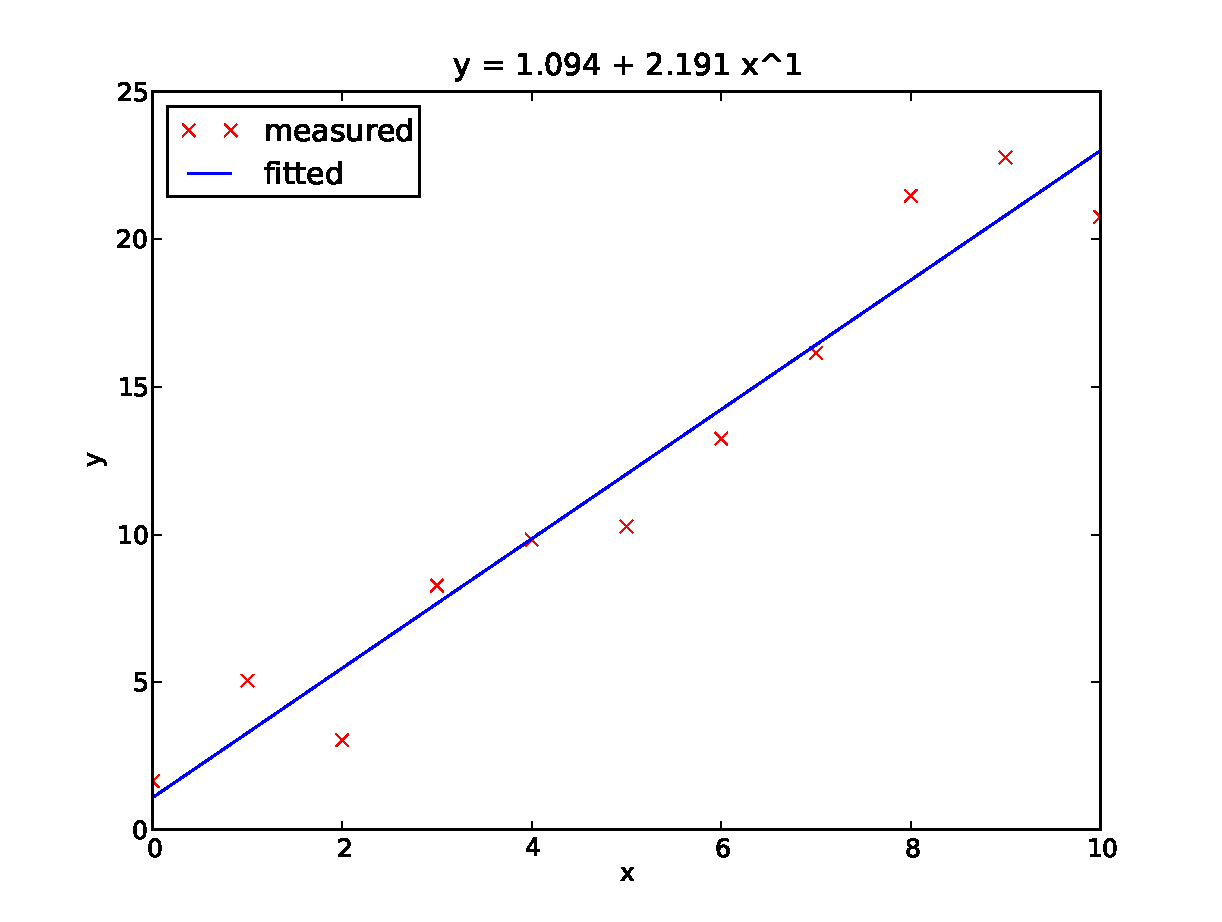
\includegraphics[width=0.5\columnwidth]{polyfit-n1}\hfill
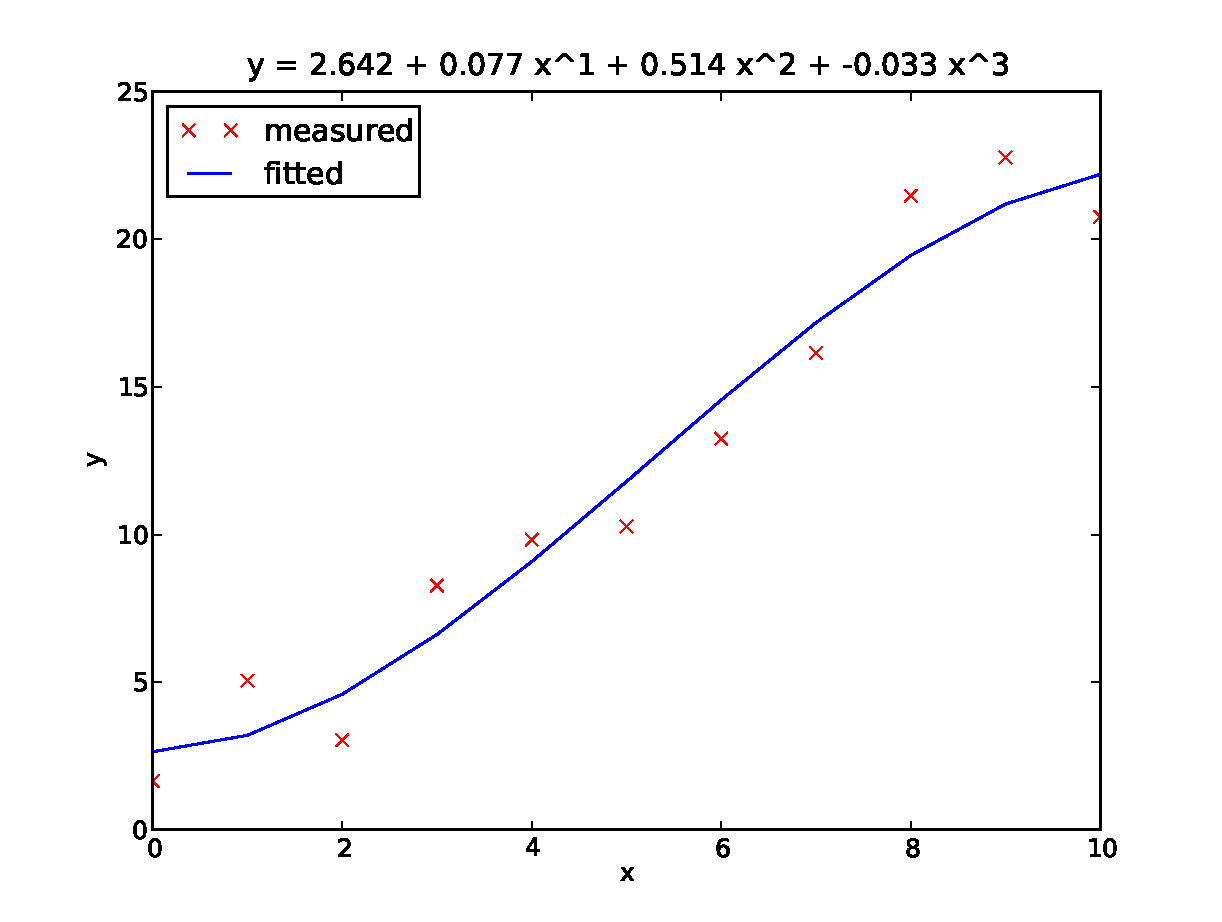
\includegraphics[width=0.5\columnwidth]{polyfit-n3}%
\caption{Polynomial fit for noisified synthetic data using first order (left) and third order (right) polynomials.}%
\label{fig:polyfit}%
\end{figure}

In the following we continue the description with C++ but all are provided as well in Python without significant code changes.

%%%%%%%%%%%%%%%%%%%%%%%%%%%%%%%%%%%%%%%%%%%%%%%%%%%%%%%%%%%%%%%%%%%%%%%%%%%
\subsection{An own Jacobian}
{\em Example file polyfit1.cpp in the directory doc/tutorial/code/polyfit.}\\
For the latter example, the underlying Gauss-Newton scheme creates a Jacobian matrix by brute force (perturbation).
If we want to apply an own algorithm we overwrite the function createJacobian() in the modelling class by using the matrix $\A$ from (\ref{eq:yAx}):
\begin{lstlisting}[language=C++,morekeywords={RMatrix,RVector,size_t}]
    void createJacobian( RMatrix & jacobian, const RVector & model ) {
        jacobian.resize( x_.size(), nc_ );
        for ( size_t i = 0 ; i < nc_ ; i++ )
            for ( size_t j = 0 ; j < x_.size() ; j++ )
                jacobian[ j ][ i ] = pow( x_[ j ], i );
    }
\end{lstlisting}

The result of the inversion is of course the same as before.
Note that the resize function checks for the right size and allocates space if necessary.

Alternatively we might to use other minimisation methods even though it is not necessary for this example.
\sperre (Steepest descent, NLCG, Quasi-Newton)

Note that \lstinline|RInversion| is an instance of the template class \lstinline|Inversion< ValueType, MatrixType >| with the value type \lstinline|double| and the matrix type \lstinline|RMatrix|\footnote{RMatrix is a full matrix of real (double) values.}.
One can, of course, use other types, e.g. the complex vector/matrix \lstinline|CVector/CMatrix|. 
For many problems the jacobian matrix has only few entries and can be approximated by a sparse matrix.
Therefore the matrix type \lstinline|RSparseMapMatrix| exists, which is itself an instance of a template type with \lstinline|long int| index and double values. 
The corresponding inversion is called \lstinline|RInversionSparse|.
